\section{Experimental Results}\label{sec:calibmatsults}
\paragraph*{Experimental Setup}In our results we used a 8x6 calibration board with 25mm squares when underwater, and a 7x6 calibration board with 29mm squares when on air. We found the use of an odd by even size calibration board avoided the possible problem of upside down corner detection. In our underwater footage this did not interfere with our underwater results so our old set up still used. The board was printed on waterproof paper and glued onto an acrylic board as smoothly as possible to avoid any extra noise. 

\begin{figure*}[hp]
	\centering
	\subfloat[Non-filtered underwater dataset without SuperView]{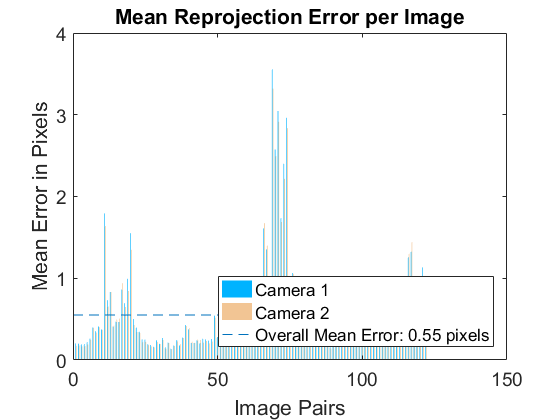
\includegraphics[width=.49\textwidth]{figures/no_sup_unw_before}}
	\subfloat[Filtered underwater dataset without SuperView]{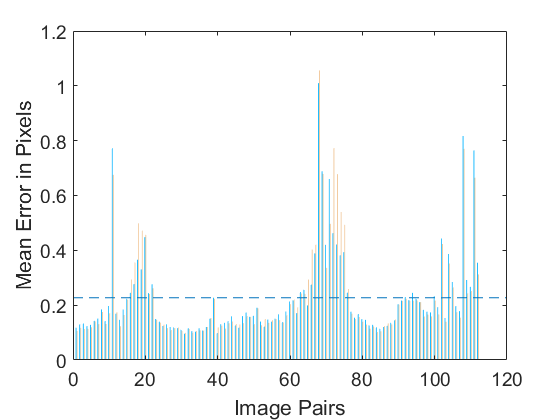
\includegraphics[width=.49\textwidth]{figures/no_sup_unw_after}}
	
	\subfloat[Non-filtered underwater dataset with SuperView]{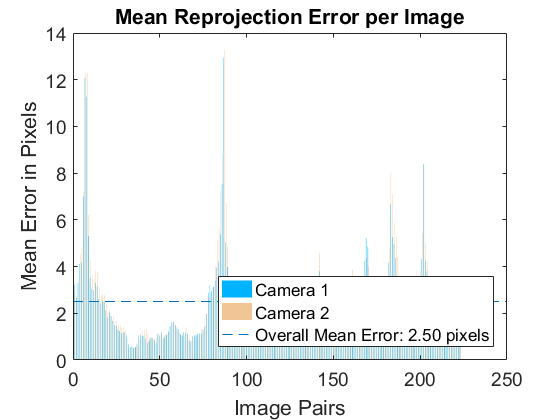
\includegraphics[width=.49\textwidth]{figures/with_sup_unw_before}}
	\subfloat[Filtered underwater dataset with SuperView]{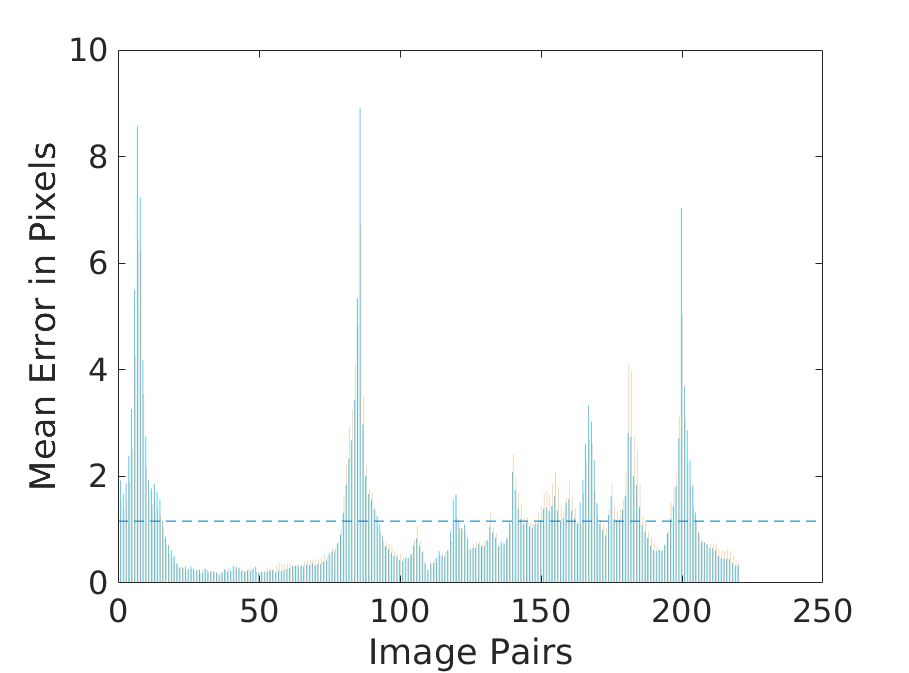
\includegraphics[width=.49\textwidth]{figures/with_sup_unw_after_fix}}
	\caption{Calibration results using MATLAB on underwater datasets. On the left column, results by using all the images, on the right column, results by filtering the dataset using the outlier removal method.\label{fig:MATresults}}
\end{figure*}

\begin{figure*}[hp]
	\centering
	\subfloat[Non-filtered above water dataset without SuperView]{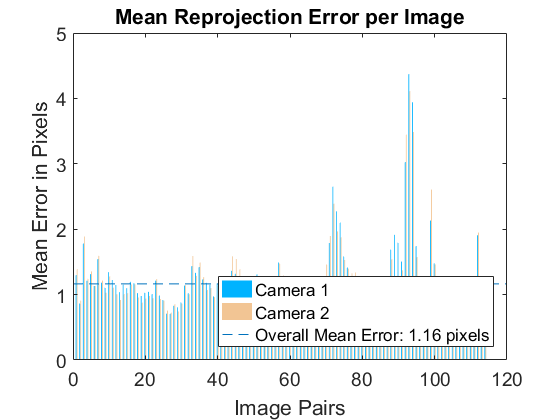
\includegraphics[width=.49\textwidth]{figures/no_sup_abvwat_before}}
	\subfloat[Filtered above water dataset without SuperView]{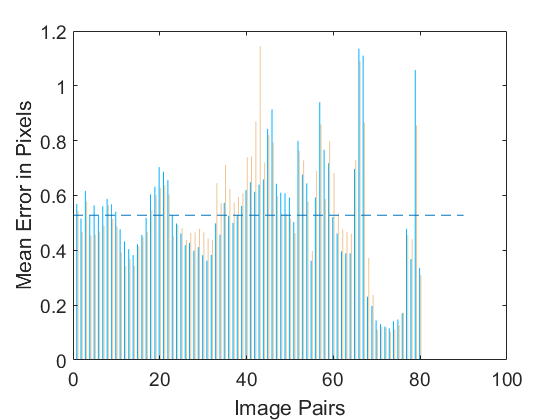
\includegraphics[width=.49\textwidth]{figures/no_sup_abvwat_after}}
	
	\subfloat[Non-filtered above water dataset with SuperView]{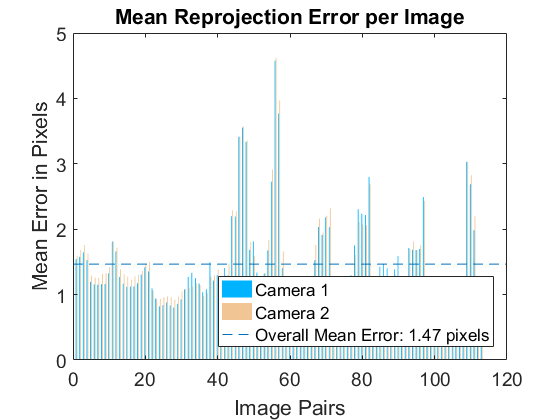
\includegraphics[width=.49\textwidth]{figures/with_sup_abvwat_before}}
	\subfloat[filtered above water dataset with SuperView]{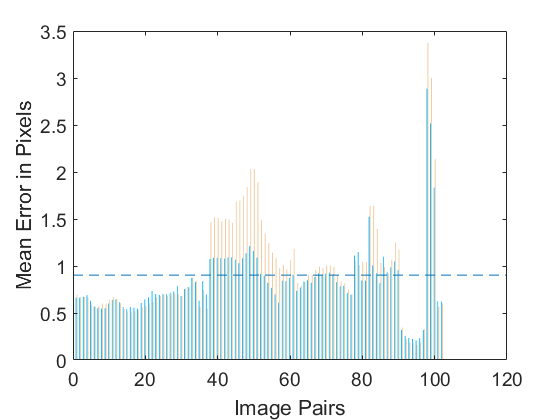
\includegraphics[width=.49\textwidth]{figures/with_sup_abvwat_after}}
	\caption{Calibration results using MATLAB on above water datasets. On the left column, results by using all the images, on the right column, results by filtering the dataset using the outlier removal method.\label{fig:MATresults2}}
\end{figure*}

\paragraph*{Calibration Procedure and Results}Using the left and right frames extracted from our calibration video, the images were run through the MATLAB Computer Vision system Toolbox Stereo Camera Calibrator upon which a result was determined. The reprojection error graph was examined in order to identify image pairs that exceeded the average image pair mean. These pairs were then removed from the input image list and the process was rerun. This happened repeatedly until either the total reprojection error fell within a specified reasonable range, or the image pair set became to small for meaningful calculations to be done. 

Using this method, we were able to calibrate a GoPro camera recording in SuperView mode with reprojection error of 0.9 on air and 0.51 underwater, compared to an error of 2.5 on air and 1.5 underwater without any outlier removal, as seen in Fig. \ref{fig:MATresults}.

Fig. \ref{fig:MATresults} compares the reprojection error results of image sets both with and without SuperView and both above and below water. 
In each case, calibration parameters were determined using a subset of full input data set---training phase---where the outliers had been removed. These parameters were then used to calculate the reprojection error of the full set once again---validation phase. 
Note that, in MATLAB, the function provided that recovers the extrinsics given the set of 2D-3D points of the checkerboard is based on a closed form formulation, while the one used inside the function for estimating the camera parameters is using a numerical optimization algorithm. As such, reprojection errors calculated on the same images from the training phase and the validation phase could be slightly different. In our experiments it was around 1-2 pixels. As such, we formulated the recovery of the extrinsics as a numerical optimization problem and we compute the error using a numerical optimization algorithm.
It can be observed that the mean pixel error is lower on the full set when the parameters from the image subset are used. Many plots still have outlier cases which result from a few possibilities. One cause is that while the corners were all detected by the corner detector, there was motion blur that skewed the actual location of the points. A second cause is the SuperView dynamic stretching that pulls the corner points outward near the edges. This effect is not completely eliminated after calibration which signifies features very close to the edge of the scene are not usable in any future processes. A future study might evaluate the region for which undistorted SuperView images remain undetected by the dynamic stretching. Comparing the results of image sets above and below water, underwater sets had a number of more sharp outlier cases. This is most likely the results of the difficulty in actually acquiring underwater calibration footage. The two domains did both had success in producing low reprojection error. In our case we even got slightly better error results from using SuperView underwater compared to above water, possibly because of the additional water distortion effect.